\documentclass[12pt,letterpaper]{article}
\usepackage[margin=.63in,headheight=15pt,headsep=19pt,footskip=25pt]{geometry}
\usepackage{tikz,fancyhdr,enumitem}
\usetikzlibrary{arrows.meta}
\renewcommand{\familydefault}{\sfdefault}
\pagestyle{fancy}\fancyhf{}\renewcommand{\headrulewidth}{.4pt}
\fancyhead[L]{\small Week 18 / Hidden changes encore / Grades 2--5}
\fancyfoot[L]{\small Bellingham Math Circle / Week 18 / W18-BON-v1}\fancyfoot[R]{\small\thepage}
\setlength{\parindent}{0pt}\setlength{\parskip}{9pt}
\newcommand{\problem}[2]{\textbf{Problem #1:} #2\par}
\newcommand{\strip}[2][1]{\begin{tikzpicture}[x=25mm,y=25mm,scale=#1]
\foreach \v [count=\i from 0] in {#2}{\draw (\i,0) rectangle +(1,1);\node[font=\scriptsize] at (\i+.5,1.17){\pgfmathparse{int(\i+1)}\pgfmathresult};\ifnum\v=1\fill (\i+.5,.5) circle (.19);\else\ifnum\v=0\draw (\i+.5,.5) circle (.19);\else\ifnum\v=2\node at (\i+.5,.5){\large ?};\fi\fi\fi}\end{tikzpicture}}
\newcommand{\lines}[1]{\foreach \i in {1,...,#1}{\par\vspace{10pt}\hrulefill}\par}
\newcommand{\arraymat}[2][1]{\begin{tikzpicture}[x=25mm,y=25mm,scale=#1]
\fill[gray!12] (3,0) rectangle (4,4);\fill[gray!12] (0,0) rectangle (4,1);
\draw[step=1] (0,0) grid (4,4);\draw[very thick] (3,0)--(3,4) (0,1)--(4,1);
\foreach \x in {1,2,3}{\node[font=\small] at (\x-.5,4.23){\x};}\node[font=\small] at (3.5,4.23){check};
\foreach \y/\lab in {3.5/1,2.5/2,1.5/3,.5/check}{\node[font=\small,anchor=east] at (-.12,\y){\lab};}
\foreach \row [count=\j from 0] in {#2}{\foreach \v [count=\i from 0] in \row{\ifnum\v=1\fill (\i+.5,3.5-\j) circle (.18);\else\ifnum\v=0\draw (\i+.5,3.5-\j) circle (.18);\fi\fi}}
\end{tikzpicture}}
\newcommand{\smallcheckmat}[1]{\begin{tikzpicture}[x=10mm,y=10mm]
\fill[gray!12] (2,0) rectangle (3,3);\fill[gray!12] (0,0) rectangle (3,1);
\draw[step=1] (0,0) grid (3,3);\draw[very thick] (2,0)--(2,3) (0,1)--(3,1);
\node[font=\scriptsize] at (2.5,3.22){check};\node[font=\scriptsize,anchor=east] at (-.1,.5){check};
\foreach \row [count=\j from 0] in {#1}{\foreach \v [count=\i from 0] in \row{\ifnum\v=1\fill (\i+.5,2.5-\j) circle (.15);\else\ifnum\v=0\draw (\i+.5,2.5-\j) circle (.15);\fi\fi}}
\end{tikzpicture}}
\begin{document}
Counters have a filled face and an open face. A hole cover hides a counter and keeps its position. A flip turns a counter over.

\problem{1}{Use this key. The sender chooses a message and covers exactly one position. The receiver sees the other two counters and the hole. Can the receiver always tell which message was sent? Try every hole position.}
\begin{center}\begin{tabular}{c@{\quad}c@{\qquad}c@{\quad}c}
A&\strip[.7]{0,0,0}&B&\strip[.7]{0,1,1}\\[12pt]
C&\strip[.7]{1,0,1}&D&\strip[.7]{1,1,0}
\end{tabular}\end{center}
\vspace{2pt}\lines{2}
\vspace{15pt}
\problem{2}{Make the shortest key for four messages that still works whenever one position is covered. Can a key with only two positions work? Explain why your shortest key cannot be shortened.}
\begin{center}\begin{tikzpicture}[x=13mm,y=12mm]
\foreach \y/\lab in {0/D,1/C,2/B,3/A}{\node at (-.5,\y+.45){\lab};\draw (0,\y) rectangle (10,\y+.9);}
\end{tikzpicture}\end{center}
\lines{2}
\newpage
The last counter in a row is a check counter. Set it so the whole row has an even number of filled faces. The receiver rejects a row with an odd number.

\begin{center}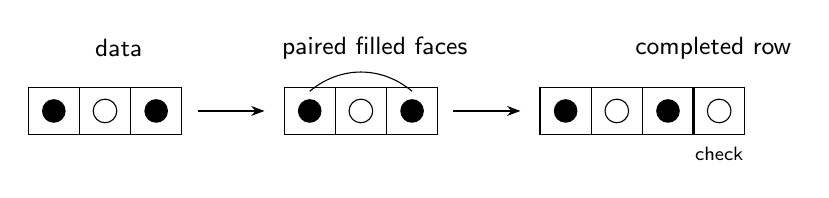
\begin{tikzpicture}[x=1cm,y=1cm]
\node at (1.15,1.1){\small data};\node at (4.4,1.1){\small paired filled faces};\node at (8.7,1.1){\small completed row};
\foreach \shift in {0,3.25}{\foreach \i/\v in {0/1,1/0,2/1}{\draw (\shift+\i*.65,0) rectangle +(.65,.6);\ifnum\v=1\fill (\shift+\i*.65+.325,.3) circle (.15);\else\draw (\shift+\i*.65+.325,.3) circle (.15);\fi}}
\draw (3.575,.55) to[bend left=40] (4.875,.55);
\draw[-{Stealth}] (2.15,.3)--(3,.3);\draw[-{Stealth}] (5.4,.3)--(6.25,.3);
\foreach \i/\v in {0/1,1/0,2/1,3/0}{\draw (6.5+\i*.65,0) rectangle +(.65,.6);\ifnum\v=1\fill (6.5+\i*.65+.325,.3) circle (.15);\else\draw (6.5+\i*.65+.325,.3) circle (.15);\fi}
\draw[very thick] (8.45,0)--(8.45,.6);\node[font=\scriptsize] at (8.775,-.25){check};
\end{tikzpicture}\end{center}

\problem{3}{Make different rows of four data counters and add a check counter. Behind a folder, your partner flips exactly one counter, anywhere in the row. Can the receiver always detect the change?}
\begin{center}\strip{3,3,3,3,3}\end{center}
\vspace{8pt}
\problem{4}{Start with a checked five-counter row. Flip each chosen counter once. Which numbers of flips can leave a row that passes the check: 1, 2, 3, 4, or 5? Find a rule that covers every starting row.}
\begin{center}\begin{tabular}{c|p{2.05in}|p{2.05in}}
flips&can pass&cannot pass\\\hline
1&&\\[12pt]\hline 2&&\\[12pt]\hline 3&&\\[12pt]\hline 4&&\\[12pt]\hline 5&&\\[12pt]\hline
\end{tabular}\end{center}
\lines{3}
\newpage
The shaded row and column contain check counters. Set them so every full row and every full column has an even number of filled faces. Keep the mat facing the same way.

\begin{center}
\begin{tabular}{c@{\quad}c@{\quad}c@{\quad}c@{\quad}c}
\small input&&\small row checks&&\small completed mat\\[5pt]
\smallcheckmat{{1,1,3},{0,1,3},{3,3,3}}&$\longrightarrow$&\smallcheckmat{{1,1,0},{0,1,1},{3,3,3}}&$\longrightarrow$&\smallcheckmat{{1,1,0},{0,1,1},{1,0,1}}
\end{tabular}
\end{center}

\problem{5}{Complete this mat. The sender then hides it and flips exactly one counter, including any check counter. Give the mat to the receiver. Can the receiver always locate the changed counter? Play again with different data and different changed positions.}
\begin{center}\arraymat{{1,1,0,3},{0,1,0,3},{1,0,0,3},{3,3,3,3}}\end{center}

\lines{2}
\newpage
\problem{6}{Start with a mat that passes every row and column check. Choose at least one counter and flip each chosen counter once. Find the fewest counters you can flip while still passing every check. Mark two different invisible patterns. Explain why fewer flips cannot work.}
\begin{center}\arraymat[.68]{{3,3,3,3},{3,3,3,3},{3,3,3,3},{3,3,3,3}}\hspace{18pt}\arraymat[.68]{{3,3,3,3},{3,3,3,3},{3,3,3,3},{3,3,3,3}}\end{center}
\lines{2}
\vspace{8pt}
\problem{7}{Start with a mat that passes every check. The sender flips exactly two counters. Can two different choices, made from the same starting mat, give the same odd rows and odd columns? Mark two such choices, or explain why there are none.}
\begin{center}\arraymat[.54]{{3,3,3,3},{3,3,3,3},{3,3,3,3},{3,3,3,3}}\hspace{30pt}\arraymat[.54]{{3,3,3,3},{3,3,3,3},{3,3,3,3},{3,3,3,3}}\end{center}
\lines{2}
\end{document}
